\newpage
\section{Arithmetic for Computer}

\subsection{Introduction}

Computer words are composed of bits. Thus one word is a vector of binary numbers. There are 32 bit/word (word) or 64 bit/word (double word) in RISC-V. 32 bits contains four bytes. 

Generic Implementation. 
\begin{enumerate}
    \item Use program counter (PC) to link to instruction address. 
    \item Fetch the instruction from memory. 
    \item The instruction tells what needs to be done. 
    \item ALU will perform the specified arithmetic operations.
\end{enumerate}

\subsection{Signed and Unsigned Numbers}

\subsubsection{Numbers and their representation}
\begin{enumerate}
    \item NUmber systems
    \begin{align*}
        (N)_k=\left( \sum_{i=m}^{n-l} b_i \cdot k^i \right)_k
    \end{align*}
    \begin{itemize}
        \item $b$: value of the digit. 
        \item $k$: radix.
        \item $n$: digits left of radix point.
        \item $m$: digits right of radix point.
    \end{itemize}
    \item Representation
    \begin{itemize}
        \item ASCII - text characters (External)
        \item Binary number (Internal)
    \end{itemize}
\end{enumerate}

\subsubsection{Number types}
\begin{itemize}
    \item  Integer numbers, unsigned
    \item Signed numbers
    \begin{itemize}
        \item Signed Number Representations: Sign Magnitud or Two's Complement
    \end{itemize}
    \item Floating point number
\end{itemize}

\subsection{Addition, subtraction and ALU}
\subsubsection{Addition \& subtraction}
\begin{itemize}
    \item Adding bit by bit, carries $\rightarrow$ next digit.
    \item Subtraction
    \begin{itemize}
        \item Directly.
        \item Addition of 2's complement.
    \end{itemize}
\end{itemize}

\subsubsection{Overflow}

Duoble sign-bits判断溢出. 

\begin{table}[H]
    \centering
    \caption{General overflow conditions}
    \begin{tabular}[c]{|c|c|c|c|}\hline
        Operation & Operand A & Operand B & Result\\ \hline
        $A+B$ & $\ge 0$ & $\ge 0$ & $<0$ \\
        $A+B$ & $< 0$ & $< 0$ & $\ge 0$ \\
        $A-B$ & $\ge 0$ & $< 0$ & $<0$ \\
        $A-B$ & $< 0$ & $\ge 0$ & $\ge 0$ \\ \hline
    \end{tabular}
\end{table}

\subsubsection{Constructing an ALU}
是一个组合, 有多种计算方式, 使用了模块化的设计. 

\begin{enumerate}
    \item A full adder
    \item Full adder Logic circuit
    \item 1 bit ALU
    \item Extended 1 bit ALU
    \begin{itemize}
        \item Subtraction
        \item Comparison
    \end{itemize}
    \item Complete ALU
    \item Complete ALU --- with Zero detector
\end{enumerate}

\subsubsection{ALU symbol \& Control}
\begin{figure}[H]
    \centering
    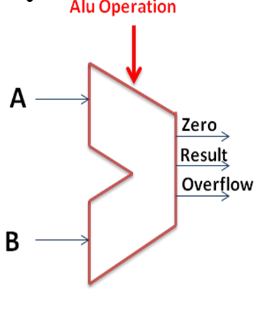
\includegraphics[width=0.189\textwidth]{CO2/Symbol of the ALU}
    \caption{Symbol of the ALU}
\end{figure}

\begin{center}
    \tablefirsthead{\hline ALU Control Lines & Function \\ \hline }
    \tablehead{\hline ALU Control Lines & Function \\ \hline }
    \tabletail{\hline}
    \tablelasttail{\hline}
	\tablecaption{Control: Function table}
    % \bottomcaption{}
    \begin{supertabular}{|c|c|}
        000 & And \\
        001 & Or \\
        010 & Add \\
        110 & Sub \\
        111 & Set on less than \\
        \textcolor{gray}{100} & \textcolor{gray}{nor} \\
        101 & srl \\
        011 & xor \\ \hline
    \end{supertabular}
\end{center}


% \begin{table}[H]
%     \centering
%     \caption{Control: Function table}
%     \begin{tabular}[c]{|c|c|}\hline
%         ALU Control Lines & Function\\ \hline
%         000 & And \\
%         001 & Or \\
%         010 & Add \\
%         110 & Sub \\
%         111 & Set on less than \\
%         \textcolor{gray}{100} & \textcolor{gray}{nor} \\
%         101 & srl \\
%         011 & xor \\ \hline
%     \end{tabular}
% \end{table}

nor被去除了(在risc里)

ALU Hardware Code ppt

\subsubsection{More information}
\begin{itemize}
    \item Speed considerations
    \item Fast adders
    \item Carry Lookahead Adder (CLA)
    \item Addition formula in CLA
    \item Carry Lookahead Development
    \item Group Block Carry Lookahead
    \item Group Carry Lookahead Logic
    \item A plumbing analogy
    \item Carry skip adder
    \item Carry select adder (CSA)
\end{itemize}

\subsection{Multiplication}

\subsubsection{Binary multiplication}
Look at current bit position

\begin{algorithm}[H]
    \caption{Binary multiplication}
    \begin{algorithmic}
        \If{multiplier is 1}
            \State add multiplicand
        \Else
            \State add 0
        \EndIf
        \State shift multiplicand left by 1 bit
    \end{algorithmic}
\end{algorithm}

\subsubsection{Multiplier V1}
\begin{enumerate}
    \item \textbf{Logic Diagram:}
    \begin{itemize}
        \item 64 bits: multiplier
        \item 128 bits: multiplicand, product, ALU
    \end{itemize}
    \item \textbf{Algorithmic rule:} Requires 64 iterations
    \begin{itemize}
        \item Addition
        \item Shift
        \item Comparison
    \end{itemize}
    Almost 200 cycles, very big, too slow!
\end{enumerate}

\subsubsection{Multiplier V2}
Real addition is performed only with 64 bits. Least significant bits of the product don't change. New idea
\begin{itemize}
    \item Don’t shift the multiplicand
    \item Instead, shift the product
    \item Shift the multiplier
\end{itemize}
ALU reduced to 64 bits. 

\begin{enumerate}
    \item \textbf{Logic Diagram:} Diagram of the V2 multiplier. Only left half of product register is changed. 
    \item \textbf{Algorithmic rule:} Addition performed only on left half of product register. Shift of product register. 
\end{enumerate}

\subsubsection{Multiplier V3}
Idea: use these lower 64 bits for the multiplier. 
\begin{enumerate}
    \item \textbf{Logic Diagram:}
    \begin{figure}[H]
        \centering
        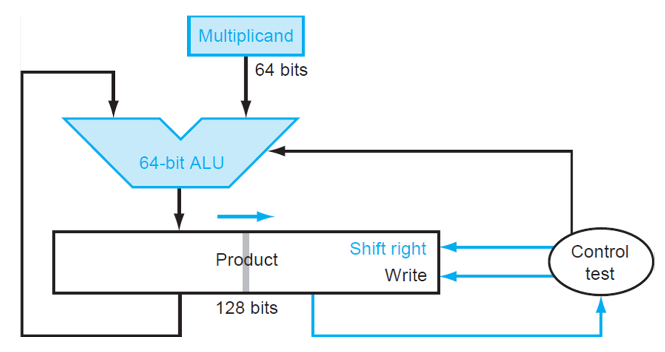
\includegraphics[width=0.309\textwidth]{CO2/Multiplier V3}
        \caption{Multiplier V3}
    \end{figure}
    
    \item \textbf{Algorithmic rule:}
    \begin{enumerate}
        \item Set product register to `0'. 
        \item Load lower bits of product register with multiplier. 
        \item Test least significant bit of product register. 
    \end{enumerate} 
\end{enumerate}

e.g. $Multiplicand \times Multiplier: 0001\times 0111$
\begin{figure}[H]
    \centering
    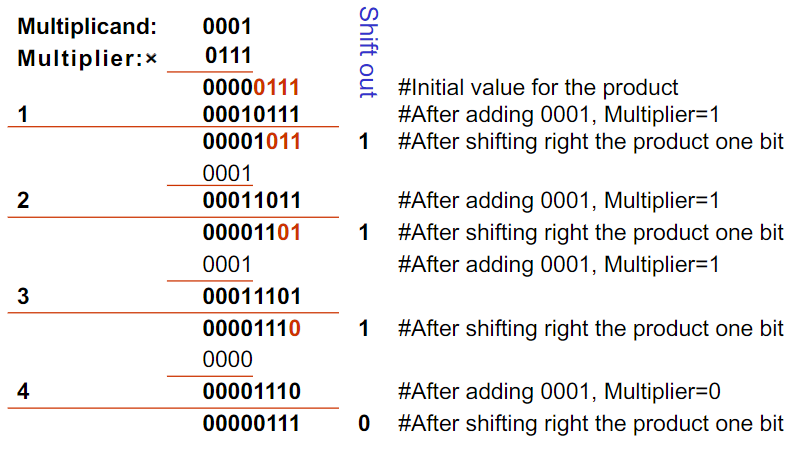
\includegraphics[width=0.479\textwidth]{CO2/Example for Multiplier V3}
    \caption{Example for Multiplier V3}
\end{figure}


\subsubsection{Signed multiplication}
\textbf{Basic approach:}
\begin{enumerate}
    \item Store the signs of the operands. 
    \item Convert signed numbers to unsigned numbers
    (most significant bit (MSB) = 0). 
    \item Perform multiplication.
    \item If sign bits of operands are equal sign bit = 0, else sign bit = 1. 
\end{enumerate}

Improved method: Booth's Algorithm. Assumption: addition and subtraction are available. 

\subsubsection{Booth's Algorithm}
\textbf{Idea:} If you have a sequence of `1's. 
\begin{itemize}
    \item subtract at first `1' in multiplier. 
    \item shift for the sequence of `1's. 
    \item add where prior step had last `1'. 
\end{itemize}

\quad

\begin{figure}[H]
    \centering
    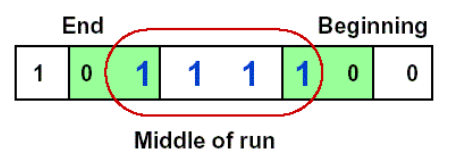
\includegraphics[width=0.309\textwidth]{CO2/Idea}
    \caption{Idea}
\end{figure}


\textbf{Result:}
\begin{itemize}
    \item Possibly less additions and more shifts. 
    \item Faster, if shifts are faster than additions. 
\end{itemize}

\subsubsection{Booth's Algorithm rule}
\textbf{Action: }
\begin{itemize}
    \item [10] subtract multiplicand from left
    \item [11] no arithmetic operation-shift add 1
    \item [01] add multiplicand to left half
    \item [00] no arithmetic operation-shift add 0
\end{itemize}
% \begin{table}[H]
%     \centering
%     % \caption{Action}
%     \begin{tabular}[c]{cl}
%         10 & subtract multiplicand from left\\
%         11 & no arithmetic operation-shift add 1\\
%         01 & add multiplicand to left half\\
%         00 & no arithmetic operation-shift add 0
%     \end{tabular}
% \end{table}
Bit${}_{-1}$=`0'. 

Arithmetic shift right: 
\begin{itemize}
    \item keeps the leftmost bit constant
    \item no change of sign bit
\end{itemize}

e.g. 
\begin{itemize}
    \item 2 * (-3) = - 6
    
    0010 * 1101 = 1111 1010
    \item 13 * (-11) = - 143
    
    01101 * 10101 = 11011 10001-->00100 01111
\end{itemize}

\subsubsection{Faster Multiplication}
Unrolls the loop. 
\begin{figure}[H]
    \centering
    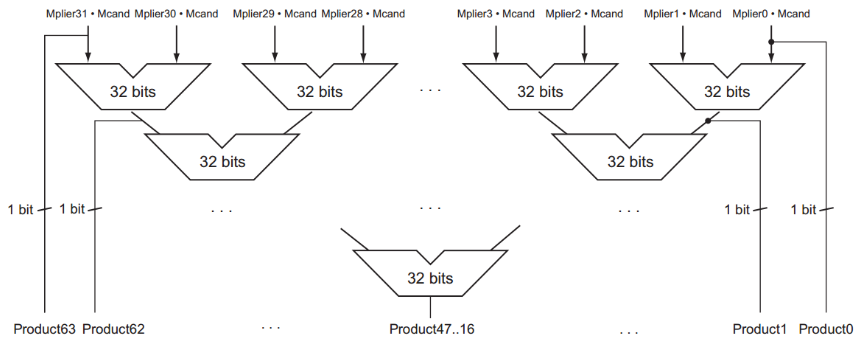
\includegraphics[width=0.479\textwidth]{CO2/Faster Multiplication}
    \caption{Faster Multiplication}
\end{figure}

\subsection{Division}

\begin{algorithm}[H]
    \caption{Division}
    \begin{algorithmic}
        \State Check for 0 divisor. 
        \Function{Long division approach}{}
            \If{divisor $\le$ dividend bits}
                \State 1 bit in quotient, subtract. 
            \Else
                \State 0 bit in quotient, bring down next dividend bit. 
            \EndIf
        \EndFunction
        \Function{Restoring division}{}
            \State Do the subtract, and if remainder goes $< 0$, add divisor back. 
        \EndFunction
        \Function{Signed division}{}
            \State Divide using absolute values. 
            \State Adjust sign of quotient and remainder as
            required. 
        \EndFunction
    \end{algorithmic}
\end{algorithm}

\subsubsection{Division V1}
\begin{enumerate}
    \item \textbf{Logic Diagram:}
    At first,the divisor is in the left half of the divisor register, the dividend is in the right half of the remainder register. Shift right the divisor register each step. 
    \item \textbf{Algorithmic rule:} 
    \begin{enumerate}
        \item Subtract divisor
        \item Depending on Result: Leaver or Restore. 
        \item Depending on Result: Write `1' or Write `0'. 
    \end{enumerate}
\end{enumerate}

\subsubsection{Modified Division}
\begin{enumerate}
    \item \textbf{Logic Diagram:} Reduction of Divisor and ALU width by half. Shifting of the remainder. Saving 1 iteration. Remainder register keeps quotient. No quotient register required.

    \begin{figure}[H]
        \centering
        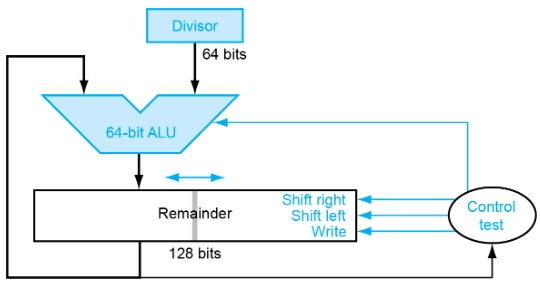
\includegraphics[width=0.479\textwidth]{CO2/Modified Division}
        \caption{Modified Division}
    \end{figure}
    One cycle per partial-remainder subtraction. Looks a lot like a multiplier. Same hardware can be used for both. 
    \item \textbf{Algorithm: }Much the same than the last one. Except change of register usage. 
\end{enumerate}

e.g. $7/2$ for Division V3, i.e. 0000 0111/0010

\begin{figure}[H]
    \centering
    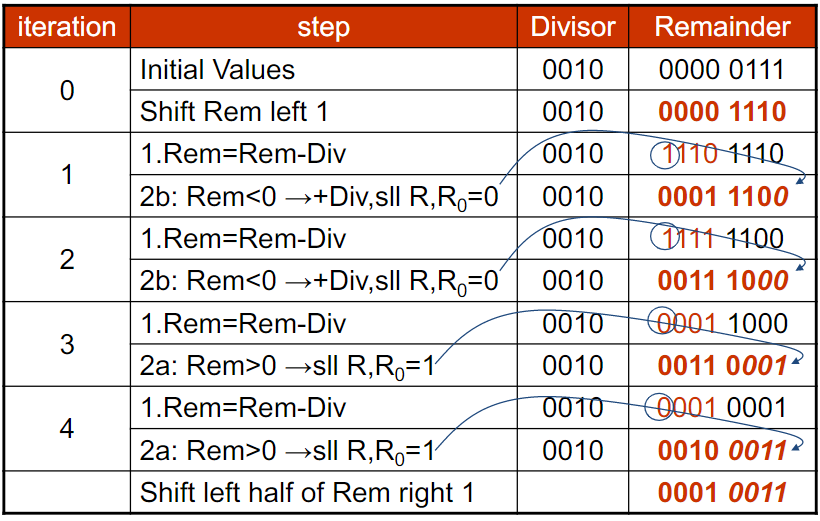
\includegraphics[width=0.479\textwidth]{CO2/Example for Division V3}
    \caption{Example for Division V3}
\end{figure}




\subsubsection{Signed division}
Keep the signs in mind for Dividend and Remainder. e.g.
\begin{itemize}
    \item $(+7) \div (+2) = +3, \, Remainder = +1$
    \item $(-7) \div (+2) = -3, \, Remainder = -1$
    \item $(+7) \div (-2) = -3, \, Remainder = +1$
    \item $(-7) \div (-2) = +3, \, Remainder = -1$
\end{itemize}

One 64 bit register : Hi \& Lo

Divide by 0 $\rightarrow$ overflow : Check by software

\subsubsection{Faster Division}
Can’t use parallel hardware as in multiplier. Subtraction is conditional on sign of remainder. 

Faster dividers (e.g. SRT division) generate multiple quotient bits per step. Still require multiple steps. 

\subsubsection{RISC-V Division}
Four instructions:
\begin{itemize}
    \item div, rem: signed divide, remainder
    \item divu, remu: unsigned divide, remainder
\end{itemize}

Overflow and division-by-zero don’t produce errors. Just return defined results. Faster for the common case of no error

\subsection{Floating point}
\textbf{Reasoning:}
\begin{itemize}
    \item Larger number range than integer rage
    \item Fractions
    \item Numbers like $e$ and $\pi$
\end{itemize}

\textbf{Representation:}
\begin{itemize}
    \item Sign
    \item Significand
    \item Exponent
    \item More bits for significand: more accuracy
    \item More bits for exponent: increases the range
\end{itemize}

\textbf{Form:} Normalised $3.634\times 10^{36}$. 

\textbf{Binary notation:} Normalised $1.xxxxx \times 2^{yyyyy}$. 

\subsubsection{Standardised format IEEE 754} 
\begin{itemize}
    \item Single precision: 8 bit exp, 23 bit significand. 
    \item Double precision: 11 bit exp, 52 bit significand. 
\end{itemize}

\begin{table}[H]
    \centering
    \caption{Single precision}
    \begin{tabular}[c]{|c|lcr|lcr|}\hline
        31 & 30 & $\dots\dots$ & 23 & 22 & $\dots\dots$ & 0 \\ \hline
        S & & exponent & & & fraction & \\ \hline
        \multicolumn{1}{c}{1 bit} & \multicolumn{3}{c}{8 bit} & \multicolumn{3}{c}{23 bit}\\ 
    \end{tabular}
\end{table}

\begin{table}[H]
    \centering
    \caption{Double precision}
    \begin{tabular}[c]{|c|lcr|lcr|}\hline
        31 & 30 & $\dots\dots$ & 20 & 19 & $\dots\dots$ & 0 \\ \hline
        S & & exponent & & & fraction & \\ \hline
        \multicolumn{1}{c}{1 bit} & \multicolumn{3}{c}{11 bit} & \multicolumn{3}{c}{20 bit}\\ \hline
        \multicolumn{1}{|l}{31} & \multicolumn{5}{c}{fraction(continued)} & \multicolumn{1}{r|}{0} \\ \hline
    \end{tabular}
\end{table}


Leading `1' bit of significand is implicit $\rightarrow$ saves one bit. 

\textbf{Exponent is biased:}
\begin{itemize}
    \item $00\dots 000$ smallest exponent
    \item $11\dots 111$ biggest exponent
\end{itemize}
Bias \hl{127} for single precision. Bias \hl{1023} for double precision. 

Summary: 
\begin{align*}
    (-1)^{sign}\times (1+significand)\times 2^{exponent-bias}
\end{align*}

e.g.


\subsubsection{Single-Precision Range}
Exponents $00000000$ and $11111111$ reserved. 
\begin{itemize}
    \item \textbf{Smallest value}
    \begin{itemize}
        \item Exponent: $00000001 \Rightarrow 1-127=-126$
    \end{itemize}
    \item \textbf{Largest value}
\end{itemize}

\subsubsection{Double-Precision Range}

\subsubsection{Floating-Point Precision}
\textbf{Relative precision:} all fraction bits are significant. 
\begin{itemize}
    \item Single: $\approx 2^{-23}$. Equivalent to $23\times \log_10 2 \approx 23 \times 0.3 \approx 6$ decimal digits of precision. 
    \item Double: $\approx 2^{-52}$. Equivalent to $52\times \log_10 2 \approx 52 \times 0.3 \approx 16$ decimal digits of precision.
\end{itemize}

\subsubsection{Limitations}
\begin{itemize}
    \item Overflow: The number is too big to be represented. 
    \item Underflow: The number is too small to be represented. 
\end{itemize}

\subsubsection{Infinities and NaNs}
\begin{itemize}
    \item $\pm$Infinity: Exponent=$111\dots 1$, Fraction=$000\dots0$
    
    Can be used in subsequent calculations, avoiding need for overflow check. 
    \item Not-a-Number (NaN): Exponent=$111\dots 1$, Fraction$\ne 000\dots0$
    
    Indicates illegal or undefined result. e.g. $\frac{0.0}{0.0}$.  
\end{itemize}

\subsubsection{Floating point addition}
\begin{enumerate}
    \item Alignment
    \item The proper digits have to be added. Addition of significand
    \item Normalisation of the result
    \item Rounding
\end{enumerate}

e.g. 0.5+(-0.4375) in binary
\begin{align*}
    0.5_{10}&=1.000_2\times2^{-1}\\
    -0.4375_2&=-1.110_2\times 2^{-2}
\end{align*}
\begin{enumerate}
    \item The fraction with lesser exponent is shifted right until matches
    \begin{align*}
        -1.110_2 \times 2^{-2} \rightarrow -0.111_2\times 2^{-1}
    \end{align*}
    \item Add the significands
    \begin{align*}
        1.000_2\times 2^{-1}\\
        \underline{+) - 0.111_2\times 2^{-1}}\\
        0.001_2\times 2^{-1}
    \end{align*}
    \item Normalize the sum and checking for overflow or underflow
    \begin{align*}
        0.001_2\times 2^{-1} \rightarrow 1.000_2\times 2^{-4}
    \end{align*}
    \item Round the sum
    \begin{align*}
        1.000_2\times 2^{-4}=0.0625_{10}
    \end{align*}
\end{enumerate}

\textbf{Logic Diagram:}

\begin{figure}[H]
    \centering
    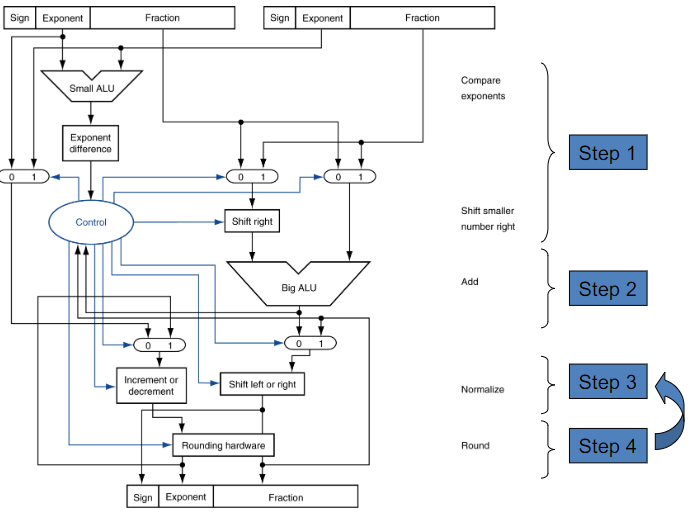
\includegraphics[width=0.39\textwidth]{CO2/Floating point addition Logic Diagram}
    \caption{Logic Diagram}
\end{figure}

\subsubsection{Multiplication}
Composition of number from different parts $\rightarrow$ separate handling. 
\begin{align*}
    (s_1 \times 2^{e_1-bias})\times(s_2\times 2^{e_2-bias})=(s_1\times s_2)\times 2^{e_1+e_2-bias}
\end{align*}

\textbf{Logic Diagram:}

\begin{figure}[H]
    \centering
    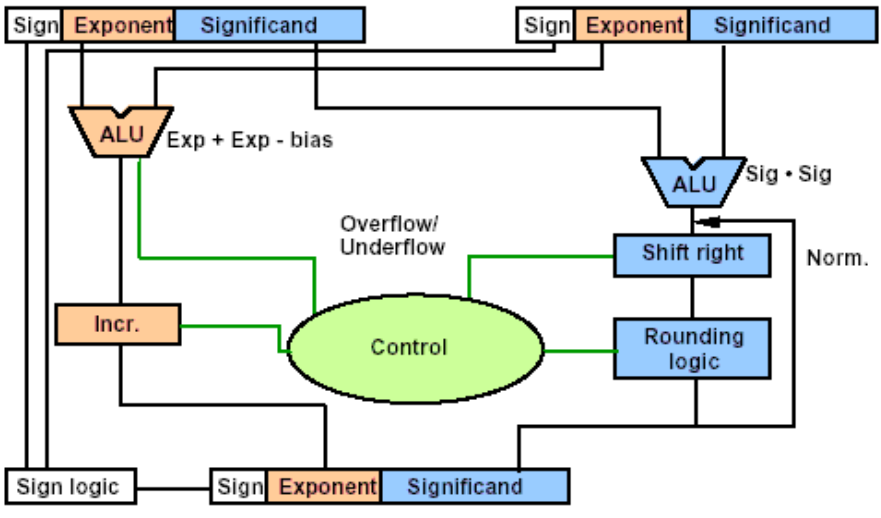
\includegraphics[width=0.309\textwidth]{CO2/Multiplication Logic Diagram}
    \caption{Logic Diagram}
\end{figure}




\textbf{Algorithmic rule:}
\begin{enumerate}
    \item Add exponents
    \item Multiply the significands
    \item Normalise
    \item Over- underflow
    \item Rounding
    \item Sign
\end{enumerate}

\subsubsection{Division --- Brief}
\begin{enumerate}
    \item Subtraction of exponents
    \item Division of the significants
    \item Normalisation
    \item Runding
    \item Sign
\end{enumerate}

\subsubsection{Accurate Arithmetic}
IEEE Std 754 specifies additional rounding control: 
\begin{itemize}
    \item Extra bits of precision (guard, round, sticky)
    \begin{itemize}
        \item Guard: the first of two extra bits.
        \item Round: method to make the immediate\\ floating-point result fit the floating-point format.
    \end{itemize}
    \item Choice of rounding modes
    \item Allows programmer to fine-tune numerical behavior of a computation. 
\end{itemize}

Not all FP units implement all options. Not all FP units implement all options. 

Trade-off between hardware complexity, performance, and market requirements.

Units in the last place(ulp): The number of bits in error in the least significant bits of the significant between the actual number and the number that can be represented.